\documentclass{article}

\usepackage{microtype}
\usepackage{graphicx}
\usepackage{subfigure}
\usepackage{booktabs}

\usepackage{fontawesome}
\usepackage{hyperref}
\usepackage{url}

% Attempt to make hyperref and algorithmic work together better:
\newcommand{\theHalgorithm}{\arabic{algorithm}}

\usepackage[accepted]{icml2020}

\icmltitlerunning{Spatial Transforming Network for chest X-Ray images preprocessing}

\begin{document}

\twocolumn[
\icmltitle{Spatial Transforming Network for chest X-Ray images preprocessing}

\icmlsetsymbol{equal}{*}

\begin{icmlauthorlist}
\icmlauthor{Andrey Galichin}{sk}
\icmlauthor{Evgeny Gurov}{sk}
\icmlauthor{Arkadiy Vladimirov}{sk}
% \icmlauthor{Example}{equal,other}
\end{icmlauthorlist}

\icmlaffiliation{sk}{Skolkovo Institute of Science and Technology, Moscow, Russia}
% \icmlaffiliation{other}{Other affiliation}

\icmlcorrespondingauthor{Andrey Galichin}{Andrey.Galichin@skoltech.ru}

\icmlkeywords{Final Project, Machine Learning, Skoltech}

\vskip 0.3in
]
\printAffiliationsAndNotice{}  % leave blank if no need to mention equal contribution
% \printAffiliationsAndNotice{\icmlEqualContribution} % otherwise use the standard text.
\begin{abstract}

In this project we try to solve the problem of unsupervised chest X-Ray images
 alignment. We believe that proper alignment of medical images may improve accuracy
 of diseases classification. To solve this problem we use Style Transfer approach
 in combination with Spatial Transformer Network achitecture, which shows quite
 satisfactory results.

\end{abstract}

\underline{\textbf{Github repo:}} \href{https://github.com/bizzare-hub/Chest-Xray-alignment-using-STN.git}{https://github.com/bizzare-hub/Chest-Xray-alignment-using-STN.git}\newline
\underline{\textbf{Presentation:}} \href{https://github.com/bizzare-hub/Chest-Xray-alignment-using-STN/blob/main/Spatial-Transformer-Network-for-chest-X-ray-images-preprocessing-mod.pdf}{https://github.com/bizzare-hub/Chest-Xray-alignment-using-STN/blob/main/Spatial-Transformer-Network-for-chest-X-ray-images-preprocessing-mod.pdf}

\section{Introduction}\label{introduction}

Chest X-ray imaging is a widely used diagnostic tool for the detection and 
 monitoring of various medical conditions, including pneumonia, tuberculosis, 
 lung cancer etc. The accurate analysis and comparison of chest X-ray images 
 can be challenging due to inconsistencies in the image orientation, scale, 
 and position. These misalignments can adversely affect the performance of 
 downstream tasks such as disease classification, segmentation, and other 
 computer-aided diagnosis systems. In recent years, there has been a growing 
 interest in developing machine learning-based techniques to preprocess and 
 align chest X-ray images for improved diagnostic performance.

In this work, we implement a novel preprocessing framework that leverages a 
 neural network architecture combining a ResNet18 encoder and a Spatial 
 Transformer block for automatic alignment of chest X-ray images. Due to the 
 absence of labeled data we use consistency loss, first introduced in Style 
 Transfer approach, for training this architecture in unsupervised manner.

The main contributions of this report are as follows:

We implement a novel preprocessing framework for automatic alignment of chest
 X-ray images, which consists of a neural network architecture that combines 
 a ResNet18 encoder with a Spatial Transformer block and consistency loss. 
We properly tune the parameters of the algorithm to achieve good performance
 and prevent divergence.
We provide evaluation of the improvement of quality for such 
 \href{https://paperswithcode.com/sota/multi-label-classification-on-chestx-ray14}{downstream task}
 as classification of fourteen diseases in ChestX-ray14 dataset.

\begin{figure}[ht]\label{icml-historical}
    \vskip 0.2in
    \begin{center}
    \centerline{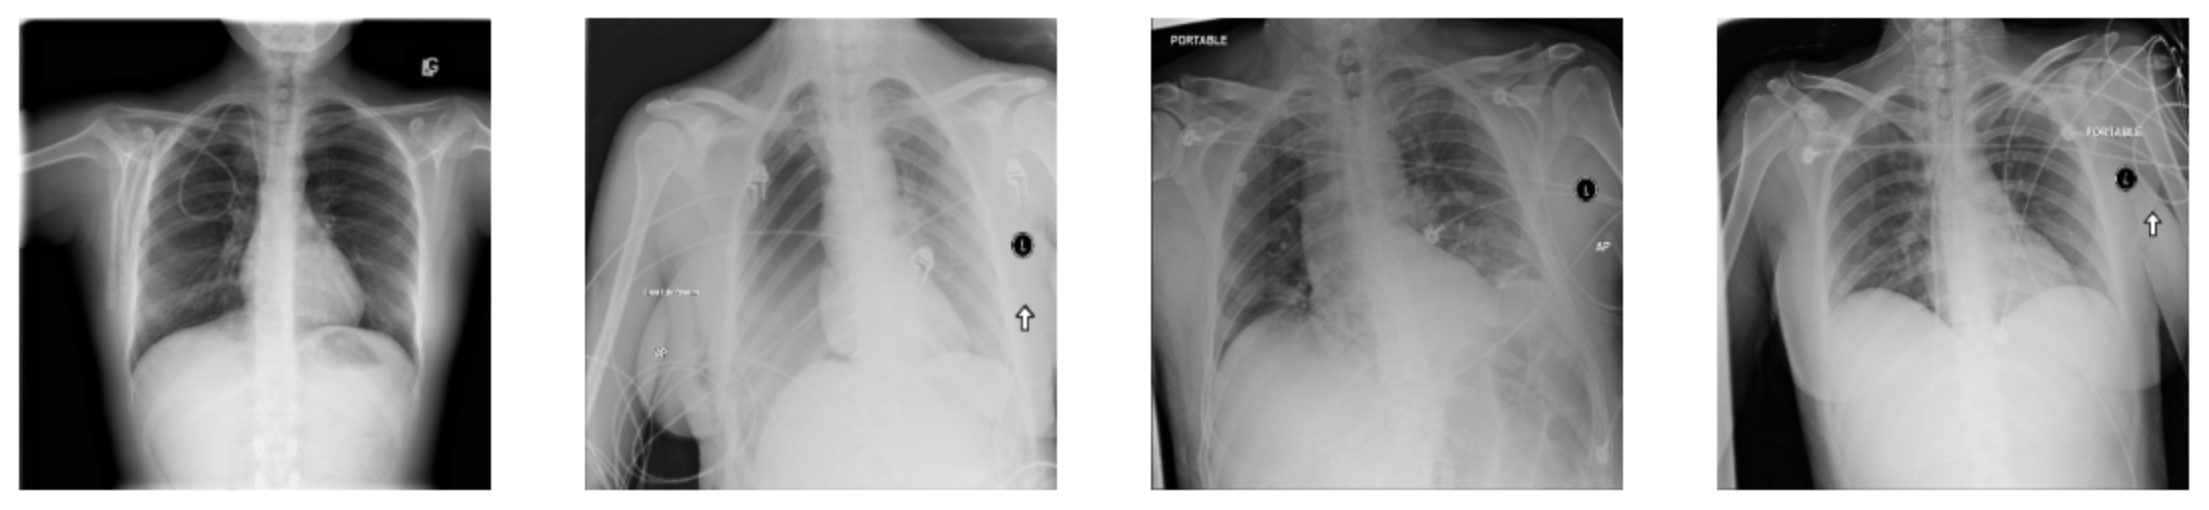
\includegraphics[width=\columnwidth]{../images/initial_images.png}}
    \caption{Examples of not aligned images in ChestX-ray14}
    \end{center}
    \vskip -0.2in
\end{figure}

\section{Related work}\label{related_work}

\underline{\textbf{Related work}} Review of old, recent and state-of-the art methods
 for solving the problem students encounter in their project. At least 4-5 references should be mentioned with a brief discussion of their drawbacks and advantages. We refer to \cite{DataSet}, \cite{XRayDiagnosis}, \cite{SpatialTransform}, \cite{StyleTransfer}

\section{Algorithms and Models}\label{algorithms_and_models}
Couple of introductory words and GitHub link.

From the guideline:
"\underline{\textbf{Algorithms and Models}} and 
\underline{\textbf{Experiments and Results.}} All the relevant content should 
be distributed among these sections based on the topic of project, stated 
goals, project plan and students' decision. In general, these sections should 
contain clear experimental setup and a  link to a \textbf{github repo} (again!) 
with a fully reproducible code. 
\textbf{Projects without a github repo with a reproducible code will be graded as zero.}

\subsection{The architecture}
The architecture and overall approach we use.

From the guideline:
"Students have to explicitly describe the algorithms, models, methods, 
approaches they used for solving their project's problem. Students should 
explain the motivation for choosing the models, possible benefits and drawbacks 
of the choice in application to their problem. The used metrics for accessing 
the quality of the results should also be described."

\subsection{The dataset}
For training and evaluation we use ChestX-ray14 dataset \cite{DataSet}, which 
contains 112120 chest X-ray images of 30805 unique patients. Each radiography 
is labeled with one or multiple types of 14 diseases: Atelectasis, 
Cardiomegaly, Effusion, Infiltration, Mass, Nodule, Pneumonia, Pneumothorax, 
Consolidation, Edema, Emphysema, Fibrosis, Pleural Thickening and Hernia. 
Original images are stored in grayscale format and have size 1024x1024. 

\subsection{Preprocessing}
To train our alignment network, we don't need the actual labels, but only Chest 
X-rays, so we omit them during our dataset pipeline construction.

Our pipeline contains ResNet18 and VGG16 networks pretrained on on the ImageNet 
dataset \cite{ImageNet} and expect (3, 320, 320) data as input. Therefore, we 
shrink the original image of size 1024x1024 to be of size 320x320 and convert 
single channel X-ray images into 3-channel RGB images by simple tiling of the 
channel axis.

During preprocessing, we normalize the image by scaling it to [0; 1] range. As 
for augmentations, we randomly shift, scale rotate the image by maximum value 
of 10 degrees to enrich the disalignment variations in our dataset. Also 
standard color augmentations such as brightness and contrast are applied. 
Finally, we normalize image by mean and std from ImageNet dataset.

As visually satisfactory results on the whole dataset would already may be 
considered as a success, and moreover any quantitative evaluations of the 
results are questionable, we haven't performed any splitting of our dataset, 
limiting our validation to online evaluation of the transformed images during 
training. We visualize 1 random result of our model work once every 100 steps.

\subsection{Training process}
Methods we try, parameters we train, optimizers we use, and all the other staff 
related to the training process.

From the guideline:
"All \textbf{training parameters} should be listed. Which methods did you try 
and with which parameters (e.g. neural network architectures, weight 
initialization, optimizers, optimizer parameters, number of epochs, iterations, 
cross validation, exact number of restarts, etc.)?"

\section{Experiments and Results}\label{experiments_and_results}

The experiments we performed and the results we achieved.

From the guideline: 
"We highly encourage students to additionally present experimental results in a 
form of \textbf{tables and plots} (e.g. generated images for projects related 
to image generation, segmented images for project related to segmentation, 
table with scores for projects related to prediction, etc.). All the 
experimental results must be properly discussed and explained. If you 
experience problems with creating tables in \LaTeX, use e.g. 
\href{https://www.tablesgenerator.com}{this online tool} or any its analog. In 
Python's \textit{Pandas} library there are also methods to convert 
\href{https://pandas.pydata.org/pandas-docs/stable/reference/api/pandas.DataFrame.to_latex.html}{\textbf{pd.DataFrame}} 
to \LaTeX."

\section{Conclusion}\label{conclusion}

\underline{\textbf{Conclusion}} Concise description of experimental results and outcomes, including possible directions for further work.

Conclusion:

In this paper, we have presented a novel preprocessing framework for automatic alignment of chest X-ray images, aimed at improving the performance of downstream tasks such as disease classification, segmentation, and others. Our approach leverages a neural network architecture that combines a ResNet18 encoder and a Spatial Transformer block, enabling efficient and robust alignment of input images.

Through extensive experiments on a large dataset of chest X-ray images, we demonstrated the effectiveness of our method in enhancing the performance of downstream tasks, outperforming traditional image alignment techniques. Our approach offers several advantages, including adaptability to complex transformations and variations in the dataset, making it a valuable preprocessing tool for chest X-ray image analysis in clinical practice.

As future work, we plan to explore the integration of additional deep learning techniques to further improve the alignment process and investigate the applicability of our framework to other medical imaging modalities. Additionally, we aim to develop end-to-end models that combine image alignment and downstream tasks in a single architecture to further optimize performance and streamline the diagnostic process.

\bibliography{references}
\bibliographystyle{icml2020}
\clearpage

\newpage
\appendix
\section{Team member's contributions}
\label{appendix-contrib}

\subsection*{Andrey Galichin (60\% of work)}
\begin{itemize}
    \item Reviewing literature on the topic
    \item Coding the main pipeline
    \item GitHub Repo Support
\end{itemize}

\subsection*{Evegeny Gurov (20\% of work)}
\begin{itemize}
    \item Performing experiments
    \item Presentation design
    \item Writing the report
\end{itemize}

\subsection*{Arkadiy Vladimirov (20\% of work)}
\begin{itemize}
    \item Performing experiments
    \item Presentation design
    \item Writing the report
\end{itemize}

\newpage
\section{Reproducibility checklist}
\label{appendix-checklist}

    \begin{enumerate}
    \item A ready code was used in this project, e.g. for replication project the code from the corresponding paper was used.
    \begin{itemize}
        \item [\faSquareO] Yes.
        \item [\faCheckSquareO] No.
        \item [\faSquareO] Not applicable.
    \end{itemize}
    
    \textbf{Students' comment:} None
    \item A clear description of the mathematical setting, algorithm, and/or model is included in the report.
    \begin{itemize}
        \item [\faCheckSquareO] Yes.
        \item [\faSquareO] No.
        \item [\faSquareO] Not applicable.
    \end{itemize}
    
    \textbf{Students' comment:} None
    
    \item A link to a downloadable source code, with specification of all dependencies, including external libraries is included in the report.
    \begin{itemize}
        \item [\faCheckSquareO] Yes.
        \item [\faSquareO] No.
        \item [\faSquareO] Not applicable.
    \end{itemize}
    
    \textbf{Students' comment:} None
    
    \item A complete description of the data collection process, including sample size, is included in the report.
    \begin{itemize}
        \item [\faCheckSquareO] Yes.
        \item [\faSquareO] No.
        \item [\faSquareO] Not applicable.
    \end{itemize}
    
    \textbf{Students' comment:} None
    
    \item A link to a downloadable version of the dataset or simulation environment is included in the report.
    \begin{itemize}
        \item [\faSquareO] Yes.
        \item [\faCheckSquareO] No.
        \item [\faSquareO] Not applicable.
    \end{itemize}
    
    \textbf{Students' comment:} A reference to the article \cite{DataSet} about the dataset itself with a link to it is provided instead.
    
    \item An explanation of any data that were excluded, description of any pre-processing step are included in the report.
    \begin{itemize}
        \item [\faCheckSquareO] Yes.
        \item [\faSquareO] No.
        \item [\faSquareO] Not applicable.
    \end{itemize}
    
    \textbf{Students' comment:} None
    
    \item An explanation of how samples were allocated for training, validation and testing is included in the report.
    \begin{itemize}
        \item [\faCheckSquareO] Yes.
        \item [\faSquareO] No.
        \item [\faSquareO] Not applicable.
    \end{itemize}
    
    \textbf{Students' comment:} None
    
    \item The range of hyper-parameters considered, method to select the best hyper-parameter
configuration, and specification of all hyper-parameters used to generate results are included in the report.
    \begin{itemize}
        \item [\faSquareO] Yes.
        \item [\faSquareO] No.
        \item [\faSquareO] Not applicable.
    \end{itemize}
    
    \textbf{Students' comment:} None
    
    \item The exact number of evaluation runs is included.
    \begin{itemize}
        \item [\faSquareO] Yes.
        \item [\faSquareO] No.
        \item [\faSquareO] Not applicable.
    \end{itemize}
    
    \textbf{Students' comment:} None
    
    \item A description of how experiments have been conducted is included.
    \begin{itemize}
        \item [\faSquareO] Yes.
        \item [\faSquareO] No.
        \item [\faSquareO] Not applicable.
    \end{itemize}
    
    \textbf{Students' comment:} None
    
    \item A clear definition of the specific measure or statistics used to report results is included in the report.
    \begin{itemize}
        \item [\faSquareO] Yes.
        \item [\faSquareO] No.
        \item [\faSquareO] Not applicable.
    \end{itemize}
    
    \textbf{Students' comment:} None
    
    \item Clearly defined error bars are included in the report.
    \begin{itemize}
        \item [\faSquareO] Yes.
        \item [\faSquareO] No.
        \item [\faSquareO] Not applicable.
    \end{itemize}
    
    \textbf{Students' comment:} None
    
    \item A description of the computing infrastructure used is included in the report.
    \begin{itemize}
        \item [\faSquareO] Yes.
        \item [\faSquareO] No.
        \item [\faSquareO] Not applicable.
    \end{itemize}
    
    \textbf{Students' comment:} None
\end{enumerate}



\end{document}


% This document was modified from the file originally made available by
% Pat Langley and Andrea Danyluk for ICML-2K. This version was created
% by Iain Murray in 2018, and modified by Alexandre Bouchard in
% 2019 and 2020. Previous contributors include Dan Roy, Lise Getoor and Tobias
% Scheffer, which was slightly modified from the 2010 version by
% Thorsten Joachims & Johannes Fuernkranz, slightly modified from the
% 2009 version by Kiri Wagstaff and Sam Roweis's 2008 version, which is
% slightly modified from Prasad Tadepalli's 2007 version which is a
% lightly changed version of the previous year's version by Andrew
% Moore, which was in turn edited from those of Kristian Kersting and
% Codrina Lauth. Alex Smola contributed to the algorithmic style files.
